
%% ----------------------------------------------------------------
%% Thesis.tex -- MAIN FILE (the one that you compile with LaTeX)
%% ---------------------------------------------------------------- 

% Set up the document
\documentclass[a4paper, 11pt, oneside]{Thesis}  % Use the "Thesis" style, based on the ECS Thesis style by Steve Gunn
\setcounter{tocdepth}{3}
\usepackage{graphicx}
\usepackage{subcaption}
%\graphicspath{Figures/}  % Location of the graphics files (set up for graphics to be in PDF format)

% Include any extra LaTeX packages required

\usepackage[square, numbers, comma, sort&compress]{natbib}  % Use the "Natbib" style for the references in the Bibliography
\usepackage{verbatim}  % Needed for the "comment" environment to make LaTeX comments
\usepackage{vector}  % Allows "\bvec{}" and "\buvec{}" for "blackboard" style bold vectors in maths
%\hypersetup{urlcolor=blue, colorlinks=true}  % Colours hyperlinks in blue, but this can be distracting if there are many links.

%% ----------------------------------------------------------------
\begin{document}

\thispagestyle{empty}
\begin{center}
\vspace{2 cm}
\Large{\textbf{\huge Deterministic and Stochastic Optimal Control of a Batch Cooling Crystallizer}\\

\normalsize
\begin{figure}
\begin{center}
\vspace{3 cm}

\includegraphics[width=2in]{logo.png}
\vspace{2 cm}
\end{center}
\end{figure}
\vspace{3 cm}
Submitted by
\\\textbf{{\Large Tushar Gupta (13CH30023)}}\\
\vspace{3cm}
Under the guidance of\\
{\Large \textbf{Prof. Debasis Sarkar}}\\
Department of Chemical Engineering,\\
Indian Institute of Technology Kharagpur,\\
Kharagpur 721302, India
\end{center}
\frontmatter      % Begin Roman style (i, ii, iii, iv...) page numbering

% Set up the Title Page
%\title  {Optimal Control of Seeded Batch Crystallizer}
%\authors  {\texorpdfstring
            %{{\textbf{Tushar Gupta(13CH30023)}}}
            %{}
            %}

%\addresses  {\groupname\\\deptname\\\univname}  % Do not change this here, instead these must be set in the "Thesis.cls" file, please look through it instead
%\date       {\today}
%\subject    {}
%\keywords   {}

\clearpage
%% ----------------------------------------------------------------

\setstretch{1.3}  % It is better to have smaller font and larger line spacing than the other way round

% Define the page headers using the FancyHdr package and set up for one-sided printing
\fancyhead{}  % Clears all page headers and footers
\rhead{\thepage}  % Sets the right side header to show the page number
\lhead{}  % Clears the left side page header

\pagestyle{fancy}  % Finally, use the "fancy" page style to implement the FancyHdr headers

%% ----------------------------------------------------------------
% Declaration Page required for the Thesis, your institution may give you a different text to place here
\Declaration{

\addtocontents{toc}{\vspace{1em}}  % Add a gap in the Contents, for aesthetics

This is to certify that the project report entitled “Optimal Control of Seeded Batch Crystallizer” submitted by Tushar Gupta  (13CH30023) towards partial fulfilment for the award of the degree of Master of Technology in Chemical Engineering to the Department of Chemical Engineering of the Indian Institute of Technology Kharagpur is an original bona fide research work carried out by him under my guidance and supervision and that the results contained in it have not been submitted in partial or full to any other university for the award of any degree.\\
 
 
\\
\\
\textbf{Date:} 30th April 2018
\begin{flushleft}
\textbf{Prof. Debasis Sarkar}\\
Department of Chemical Engineering,\\
Indian Institute of Technology, Kharagpur\\
\end{flushleft}
}
\clearpage  % Declaration ended, now start a new page

%% ----------------------------------------------------------------
% Certificte
%\pagestyle{empty}  % No headers or footers for the following pages

%\null\vfill
% Now comes the "Funny Quote", written in italics
%\textit{``Write a funny quote here.''}

%\begin{flushright}
%If the quote is taken from someone, their name goes here
%\end{flushright}

%\vfill\vfill\vfill\vfill\vfill\vfill\null
%\clearpage  % Funny Quote page ended, start a new page
%% ----------------------------------------------------------------

% The Abstract Page
\addtotoc{Abstract}  % Add the "Abstract" page entry to the Contents
\abstract{
\addtocontents{toc}{\vspace{1em}}  % Add a gap in the Contents, for aesthetics
Minimization of operation costs and the enhancement in product quality have been major concerns for all industrial processes. The field under study here is batch crystalllization which is affected heavily by the uncertainities in measurements and other errors. \\
The current work aims to study Deterministic and Stochastic methods for Optimum Control in batch crystallization. All the methods involve maximising an objective function by manipulating the cooling profile. At first, the Deterministic approach uses experimental kinetic parameters, which is then extended to Stochastic optimization to incorporate uncertainities in them. Lastly, a novel approach named “Polynomial Chaos Expansions” is implemented which has been applied successfully to other domains for Nonlinear Model Predictive Control but was not explored in detail in the field of batch cooled crystalllization. It successfuly includes probability distributions for the parameters into the model to provide a more robust optimization srategy.
}

\clearpage  % Abstract ended, start a new page
%% ----------------------------------------------------------------

\setstretch{1.3}  % Reset the line-spacing to 1.3 for body text (if it has changed)

% The Acknowledgements page, for thanking everyone
\acknowledgements{
\addtocontents{toc}{\vspace{1em}}  % Add a gap in the Contents, for aesthetics
With  great  pleasure  and  a  deep  sense  of  gratitude,  I  express  my indebtedness  to  \textbf{Prof. Debasis Sarkar}  for  his  invaluable  guidance  at  each  and  every  step  of  my  project  work.  His  constant flow  of ideas and inexhaustible enthusiasm has helped me overcome many hurdles that I faced in my work.\\
I  am  also  deeply  grateful  to  my  classmates,  who  exposed  me  to  the  intricacies of  relevant  topics through  proper  counseling  and  discussions  and  always  showed  great  interest  in  providing  timely support, suitable suggestions and constant encouragement.

}
\clearpage  % End of the Acknowledgements
%% ----------------------------------------------------------------

\pagestyle{fancy}  %The page style headers have been "empty" all this time, now use the "fancy" headers as defined before to bring them back


%% ----------------------------------------------------------------
\lhead{\emph{Contents}}  % Set the left side page header to "Contents"
\tableofcontents  % Write out the Table of Contents

%% ----------------------------------------------------------------
%\lhead{}  % Set the left side page header to "List if Figures"
%\listoffigures  % Write out the List of Figures

%% ----------------------------------------------------------------
%\lhead{\emph{List of Tables}}  % Set the left side page header to "List of Tables"
%\listoftables  % Write out the List of Tables

%% ----------------------------------------------------------------
%\setstretch{1.5}  % Set the line spacing to 1.5, this makes the following tables easier to read
%\clearpage  % Start a new page
%\lhead{\emph{Abbreviations}}  % Set the left side page header to "Abbreviations"
%\listofsymbols{ll}  % Include a list of Abbreviations (a table of two columns)
%{
% \textbf{Acronym} & \textbf{W}hat (it) \textbf{S}tands \textbf{F}or \\
%\textbf{LAH} & \textbf{L}ist \textbf{A}bbreviations \textbf{H}ere \\

%}

%% ----------------------------------------------------------------
%\clearpage  % Start a new page
%\lhead{}  % Set the left side page header to "Physical Constants"
%\listofconstants{lrcl}  % Include a list of Physical Constants (a four column table)
%{
% Constant Name & Symbol & = & Constant Value (with units) \\
%Speed of Light & $c$ & $=$ & $2.997\ 924\ 58\times10^{8}\ \mbox{ms}^{-\mbox{s}}$ (exact)\\

%}

%% ----------------------------------------------------------------
%\clearpage  %Start a new page
%\lhead{\emph{Symbols}}  % Set the left side page header to "Symbols"
%\listofnomenclature{lll}  % Include a list of Symbols (a three column table)
%{
% symbol & name & unit \\
%$a$ & distance & m \\
%$P$ & power & W (Js$^{-1}$) \\
%& & \\ % Gap to separate the Roman symbols from the Greek
%$\omega$ & angular frequency & rads$^{-1}$ \\
%}
%% ----------------------------------------------------------------
% End of the pre-able, contents and lists of things
% Begin the Dedication page

%\setstretch{1.3}  % Return the line spacing back to 1.3

%\pagestyle{empty}  % Page style needs to be empty for this page
%\dedicatory{For/Dedicated to/To my\ldots}

%\addtocontents{toc}{\vspace{2em}}  % Add a gap in the Contents, for aesthetics


%% ----------------------------------------------------------------
\mainmatter	  % Begin normal, numeric (1,2,3...) page numbering
\pagestyle{fancy}  % Return the page headers back to the "fancy" style

% Include the chapters of the thesis, as separate files\\

% Just uncomment the lines as you write the chapters

\chapter{Introduction}
Batch crystallization is widely used in chemical, pharmaceutical, photographic, and other manufacturing processes for the preparation of crystalline products with several desirable attributes. \\
The batch system helps to obtain a narrower Particle size distribution (PSD) with high crystal purity. The crystallization process has an influence on the downstream processing and, hence, reproducible PSD in each operation is of prime importance. Thus, it is essential to find the variables affecting the process and control them within an acceptable range, so as to satisfy the final product quality requirements.
Considering the operation of crystallizers, a batch process is preferable as a larger mean crystal size and narrower Crystal size distribution (CSD) can be achieved. In general, the CSD which is typically characterized by the mean and variance of crystal size is a key property to control this process because it directly affects final product qualities. Therefore, finding effective control strategy to obtain the crystals with a desired CSD is significant in order for improving the performance of batch crystallization processes and at the same time reducing difficulties in downstream processing.
In the following work we formulate the problem using the population balance equations and obtain the solution for the optimal Temperature profile using Deterministic and Probabilistic methods 


\paragraph{Deterministic Optimal Control} 

Quisque tristique urna in lorem laoreet at laoreet quam congue. Donec dolor turpis, blandit non imperdiet aliquet, blandit et felis. In lorem nisi, pretium sit amet vestibulum sed, tempus et sem. Proin non ante turpis. Nulla imperdiet fringilla convallis. Vivamus vel bibendum nisl. Pellentesque justo lectus, molestie vel luctus sed, lobortis in libero. Nulla facilisi. Aliquam erat volutpat. Suspendisse vitae nunc nunc. Sed aliquet est suscipit sapien rhoncus non adipiscing nibh consequat. Aliquam metus urna, faucibus eu vulputate non, luctus eu justo.

\paragraph{Stochastic Optimal Control}

Donec urna leo, vulputate vitae porta eu, vehicula blandit libero. Phasellus eget massa et leo condimentum mollis. Nullam molestie, justo at pellentesque vulputate, sapien velit ornare diam, nec gravida lacus augue non diam. Integer mattis lacus id libero ultrices sit amet mollis neque molestie. Integer ut leo eget mi volutpat congue. Vivamus sodales, turpis id venenatis placerat, tellus purus adipiscing magna, eu aliquam nibh dolor id nibh. Pellentesque habitant morbi tristique senectus et netus et malesuada fames ac turpis egestas. Sed cursus convallis quam nec vehicula. Sed vulputate neque eget odio fringilla ac sodales urna feugiat.
\textbf{Ito Process} and \textbf{Polynomial Chaos Expansions}
 % Introduction

% Background Literature survey


\chapter{Theory}

Crystallization is the (natural or artificial) process where a solid forms where the atoms or molecules are highly organized in a structure known as a crystal. Some of the ways which crystals form are through precipitating from a solution, melt or more rarely deposited directly from a gas. \\
Crystal shapes can include cubic, tetragonal, orthorhombic, hexagonal, monoclinic, triclinic, and trigonal. In order for crystallization to take place a solution must be "supersaturated". Supersaturation refers to a state in which the liquid (solvent) contains more dissolved solids (solute) than can ordinarily be accommodated at that temperature.

Supersaturation , can be mathematically defined as :\\
\begin{math}
\textbf{Supersaturation} \( = \Delta{C} = C - C_{s} \) \\
\textbf{Relative Supersaturation} \( = \Delta{C} / C_{s} = S\) \\

\end{math} 

C\textsubscript{s} : Concentration of solute in saturated solution \\
C :   Concentration of solute in the solution \\
S :   Supersaturation ratio \\
\paragraph{}
The crystallization process consists of two major type of kinetics, \textit{nucleation} and \textit{crystal growth} which are driven by thermodynamic properties as well as chemical properties.

\begin{itemize}
\item \textbf{Nucleation} is the step where the solute molecules or atoms dispersed in the solvent start to gather into clusters, on the microscopic scale (elevating solute concentration in a small region). These stable clusters constitute the nuclei.

\item \textbf{Crystal growth} is the subsequent size increase of the nuclei that succeed in achieving the critical cluster size. it is a dynamic process occurring in equilibrium where solute molecules or atoms precipitate out of solution, and dissolve back into solution.

\end{enumerate}
\\

Supersaturation is the practical driving forces of a crystallization process. Depending upon the conditions, either nucleation or growth may be predominant over the other, dictating crystal size.\\
Two other phenomena which are often neglected in the crystallization modelling process are \textbf{Agglomeration} and \textbf{Breakage}. Agglomeration occurs when two particles collide and stick together to form a larger particle. Breakage occurs in stirred vessels; the larger particle breaks into smaller fragments, because of attrition .


\section{Nucleation}

This is the initial process for the formation of a crystals in a solution, a liquid, or a vapour, in which a small number of ions, atoms, or molecules become arranged in a characteristic pattern of a crystalline solid, and subsequently form a site upon which additional particles are deposited as the crystal grows.\\
Nucleation requires supersaturation, which is obtained usually by a change in temperature (cooling in case of a positive gradient of the solubility curve and heating in case of a negative gradient), by removing the solvent, or by adding a drowning out agent or reaction partners. If the solution contains neither solid foreign particles or crystals of its own type, nuclei are formed only through homogeneous nucleation. If foreign particles are present then nuclei are formed through heterogeneous nucleation.\\
Both homogeneous nucleation and heterogeneous nucleation are classified as primary nucleation.


\section{Crystal Growth}

Crystal growth occurs as soon as nuclei with radius larger than the critical radius have been formed. There are many proposed mechanisms for crystal growth.\\
Diffusion theories assume that matter is deposited continuously on the crystal face at a rate proportional to the difference in concentration between the point of deposition and the bulk of the solution.\\
When dealing with crystal growth in an ionizing solute, the following steps can be distinguished :
\begin{itemize}
\item Bulk diffusion of solvated ions through the diffusion boundary layer
\item Bulk diffusion of solvated ions through adsorption layer
\item Surface diffusion of solvated or unsolvated ions
\item Partial or total desolvation of ions
\item Integration of ions into the lattice
\item Counterdiffusion through adsorption layer of water released
\item Counterdiffusion of water through the boundary layer

\end{itemize}

\textit{The slowest of these steps are rate determining.} \\

A crystal surface grow in such a way that units in a supersaturated solution are first transported by diffusion and convection and then built into the surface of the crystal by integration or an integration reaction , with the supersaturation, $\Delta{C}$, being the driving force.\\
Thus, determination of the optimal temperature or supersaturation trajectory for a seeded batch crystallizer is the most well-studied problem in chemical engineering, apart from batch reactors and batch distillation as the evolution of supersaturation in time affects almost all the kinetic phenomena occurring in the crystallization process. For example, growth can be size-independent or size-dependent; it can have a constant value or it may be a function of a thermodynamic parameter such as solubility and thus selection of appropriate kinetics is essential for accurate modelling .

 % Theory

% Modeling a batch crystallizer

\chapter{Modelling of a Seeded Batch Crystallizer}


\section{Population Balance Equation}

Analysis of a particulate system seeks to synthesize the behavior of the population of particles and its environment from the behavior of single particles in their local environments. The population is described by the density of a suitable extensive variable, usually the \textbf{number of particles}, but sometimes by other variables such as the mass or volume of particles. The usual transport equations expressing conservation laws for material systems apply to the behavior of single particles. Particulate processes are characterized by properties such as particle shape, size, surface area, mass, and product purity. \\
A population balance formulation describes the process of crystal size distribution with time most effectively. Thus, modeling of a batch crystallizer involves the use of population balances to model the crystal size prediction and the mass balance on the system can be modeled as a simple differential equation having concentration as the state variable.
The population balance can be expressed as eq :

\begin{equation} \label{populationbalance}
	\frac{\partial{n(r,t)}}{\partial{t}} + \frac{\partial{G(r,t)n(r,t)}}{\partial{r}} = B  \nolinebreak
\end{equation}
where \textbf{n} is the number density distribution, \textbf{t} is the time, \textbf{r} represents the characteristic dimension for size measurements, \textbf{G} is the crystal growth rate, and \textbf{B} is the nucleation rate. Both growth and nucleation processes describe crystallization kinetics, and their expression may vary, depending on the system under consideration.

\section{Model Equations} \label{modeleq}

In this work, the system under consideration is potassium sulfate, which has been studied earlier by Hu et al. \cite{hu}, Shi et al. \cite{shi}, and Paengjuntuek et al.\cite{paeng}. \\

Nucleation kinetics$^{(5-7)}$ are defined by :
\begin{equation}
B(t) = k_{b}\exp{\left(-E_{b}/RT \right)}\left(\frac{C - C_{s}(T)}{C_{s}(T)}\right)^{b}\mu_{3}
\end{equation}  


Growth Kinetics$^{(5-7)}$ are given by:
\begin{equation}
G(t) = k_{g}\exp{\left(-E_{g}/RT \right)}\left(\frac{C - C_{s}(T)}{C_{s}(T)}\right)^{g}
\end{equation}
where k$_{b}$ and k$_{g}$ are constants of the system, E$_{b}$ and E$_{g}$ are activation energies, and b and g are exponents of nucleation and growth, respectively. $C_{s}(T)$ is the saturation concentration at a given temperature. The following equations are used to evaluate the saturation and metastable concentrations corresponding to the solution temperature T (expressed in units of $^\circ$C)\cite{shi}.
\begin{align}
C_{s}(T) &= 6.29\times10^{-2} + 2.46\times10^{-3}T - 7.14\times10^{-6}T^{2} \\
C_{m}(T) &= 7.76\times10^{-2} + 2.46\times10^{-3}T - 8.1\times10^{-6}T^{2} \label{meta}
\end{align} 
The mass balance, in terms of concentration of the solute in the solution, is expressed as :
\begin{equation}
\frac{dC}{dt} = -3\rho{}k_{v}G(t)\mu_{2}(t)
\end{equation}
where $\rho{}$ is the density of the crystals, $k_{v}$ the volumetric shape factor, and $\mu_{2}$ is the second moment of particle size distribution (PSD).\\

Since $n(r,t)$ represents the population density of the crystals, the i-th moment of the particle size distribution(PSD) is given by :
\begin{equation} \label{moments}
\mu_{i} = \int_{0}^{\infty} r^{i}n(r,t) dr
\end{equation}

The above equations along with the Population Balance Equation represent a complete model of a seeded batch crystallizer . 
Since population balance equations are multidimensional, their implementation in control functions is tedious; hence, much research has been focused on the model order reduction methods.\\
For simplifying the solution method, we reduce the population balance equations into \textbf{Moment balance equations}(ODE). This is done by multiplying the equation (\ref{populationbalance})  with $r^{i}$ on both sides to generate the expression given by equation (\ref{moments}). It is also advantageous, since it is difficult and time-consuming to formulate an optimization problem involving PBEs. Thus, the moment method leads to a reduced-order model involving the process dynamics in batch crystallization.

%%%% Insert table of parameters

\section{Solution Methodology}

Separate moment equations are used for the seed and nuclei classes of crystals, and they are defined as : 
\begin{align}
\mu^{n}_{i} = \int_{0}^{r_{g}} r^{i}n(r,t) dr \\
\mu^{s}_{i} = \int_{r_{g}}^{\infty} r^{i}n(r,t) dr
\end{align}
n : nucleated crystal , s: seeded crystal , $r_{g}$  : critical radius separating the two \\  
Since, we ignore the agglomeration and breakage phenomena, the number of seeds added to the process ($\mu_{0}^{s}$) remain constant.\\
Fourth and higher order moments are not affected by the lower, which makes it possible for the complete process dynamics to be expressed by the first 4 moments for each of the respective crystals growth patterns.\\
The moment equations for nucleated and seeded crystals become as follows\cite{yenkie} :

\begin{enumerate}

\item Nucleated crystals\cite{hu}\cite{paeng} 
\begin{align}
\frac{d\mu_{0}^{n}}{dt} &= B(t) \\
\frac{d\mu_{i}^{n}}{dt} &= iG(t)u_{i-1}^{n}(t) \quad  i = 1,2,3
\end{align}

\item Seeded crystals\cite{hu}\cite{paeng}
\begin{align}
\frac{d\mu_{i}^{s}}{dt} &= iG(t)u_{i-1}^{n}(t) \quad  i = 1,2,3 \\
\mu_{0}^{s} &= constant
\end{align}

\end{enumerate}
The total moment is obtained as the summation $\mu_{i}^{t} = \mu_{i}^{n} + \mu_{i}^{s}$. 
The complete set of differential equations are as follows\cite{yenkie} :
\begin{align} 
\frac{dy_{1}}{dt} &= -3\rho k_{v}G(t)(y_{4}+y{8}) \\
\frac{dy_{2}}{dt} &= 0 \\
\frac{dy_{3}}{dt} &= G(t)y_{2}  \\
\frac{dy_{4}}{dt} &= 2G(t)y_{3} \\
\frac{dy_{5}}{dt} &= 3G(t)y_{4} \\
\frac{dy_{6}}{dt} &= B(t)  \\
\frac{dy_{7}}{dt} &= G(t)y_{6}  \\
\frac{dy_{8}}{dt} &= 2G(t)y_{7}  \\
\frac{dy_{9}}{dt} &= 3G(t)y_{8}  \\
\end{align} 
Here the state variables $y_{i}$ are given by : 
\begin{equation*}
y_{i} = \left[\quad C \quad \mu_{0}^{s} \quad \mu_{1}^{s}\quad \mu_{2}^{s}\quad \mu_{3}^{s}\quad \mu_{0}^{n}\quad \mu_{1}^{n}\quad \mu_{2}^{n}\quad \mu_{3}^{n}\quad\right]  
\end{equation*} % Model for the problem

% Optimal Control Problems 
\chapter{Optimal Control Problems}

\section{Deterministic Optimal Control} \label{deterministic}


\paragraph{Aim}
To find an optimal temperature trajectory, which minimizes the total volume of fine crystals, represented by the third moment of nucleated crystals ($\mu_{3}^{n}$ ) and maximizes the size of seeded crystals represented by the third moment of seeded crystals ($\mu_{3}^{s}$) in order to satisfy the product quality requirements.

\paragraph{Objective Function}
\begin{equation*}
\max_{T(t)}\lbrace{\mu_{3}^{s}(t_{f}) - \mu_{3}^{n}(t_{f})\rbrace } 
\end{equation*}
For uniformity of shape and size in the crystals in a seeded batch crystallization process, it is essential to ensure that the nucleation phenomena occurs to the minimum and mostly the seeded crystals grow to the desired size at a certain rate, which explains the nature of the objective function .

\paragraph{Active Constraints}
\begin{equation*}
C_{s}\leqslant C \leqslant C_{m}
\end{equation*}
The state variables can be represented as :
\begin{equation*}
y_{i} = \left[\quad C \quad \mu_{0}^{s} \quad \mu_{1}^{s}\quad \mu_{2}^{s}\quad \mu_{3}^{s}\quad \mu_{0}^{n}\quad \mu_{1}^{n}\quad \mu_{2}^{n}\quad \mu_{3}^{n}\quad\right]  
\end{equation*}

Thus, the complete model involving the moment equations consists of nine state equations. 

\subsection{Solution Technique : Steepest Ascent Hamiltonian}

The method involves use of the \textbf{Maximum Principle} discussed by Diwekar et al.\cite{diwekar} in detail. The algorithm of Steepest Ascent utilizes this principle using the Hamiltonian Derivative to move towards the optimum value of Temperature and maximise the objective function. \\
The formulation results in two point boundary value problem, since initial conditions for the state variables and final conditions for the adjoint variables are available. The method also involves introduction of nine additional variables, known as adjoints ($z_{i}$), corresponding to each of the state variable ($y_{i}$), which must satisfy the \textbf{Hamiltonian equation} represented by :
\begin{equation}
H &= \sum_{i = 1}^{9} z_{i}f(y_{i},t,T) 
\end{equation}
The complete problem can be described as :
\begin{align*}
&\max_{T(t)} \lbrace{ y_{5}(t_{f}) - y_{9}(t_{f})}\rbrace \\
&\frac{dy_{i}}{dt} = f(y_{i},t,T) \\
&\frac{dz_{i}}{dt} = \sum_{j=1}^{9} z_{j}\frac{\partial f(y_{i},t,T)}{\partial y_{i}} = f(y_{i},z_{i},t,T) \\
\end{align*}
with the following initial conditions:\\
$t_{0} = 0$ and $t_{f} = 1800s$ (batch time)
\begin{align*}
&y_{i}(t_{0}) = \left[ 0.1743 \quad 66.66 \quad 1.83\times10^{4}\quad 5.05\times10^{6} \quad 1.93\times10^{9} \quad 0.867 \quad 0 \quad 0 \quad 0 \right] \\
&z_{i}(t_{f}) = \left[  0 \quad 0 \quad 0 \quad 0 \quad 1 \quad 0 \quad 0 \quad 0 \quad -1 \right] 
\end{align*}
\paragraph{Algorithm}
\begin{enumerate}
\item An initial temperature $T(t) = 323 K$ is assumed for the entire time horizon.
\item The differential equations for state variables are integrated using the initial conditions for a time step of 1s .
\item The value of the adjoint variables are computed by backward integration for the same time step used in the previous.
\item For evaluation of the Hamiltonian derivative, an analytical method proposed by Benavides and Diwekar\cite{benavides},  is used in which we an additional variable corresponding to each of the state and adjoint variable is introduced.
\item The variable $\theta_{i}$ corresponds to each of the state variable $y_{i}$ and the variable $\phi_{i}$ corresponds to each of the adjoint variable $z_{i}$, respectively.
\item The Hamiltonian derivative is now calculated at each time step  as :
\begin{align}
&\theta = \frac{dy_{i}}{dT} \quad and \quad \phi_{i} = \frac{dz_{i}}{dT} \\
&\frac{dH}{dT} = \sum_{i=1}^{9} \left( \frac{dH}{dy_{i}}\right)\left(	\frac{dy_{i}}{dT} \right) + \sum_{i=1}^{9} \left(\frac{dH}{dz_{i}}\right)\left(\frac{dz_{i}}{dT} \right)
\end{align}
\item The  convergence criterion $(\frac{dH}{dT}<$ tolerance) is verified. If it is not satisfied, the temperature $T(t)$ is updated using this gradient\cite{yenkie}.
\begin{equation}
T^{new}(t) = T^{old}(t) + M\left(\frac{dH}{dT} \right)
\end{equation}
\item The concentration is evaluated  at that time step and compared with first with the saturation concentration ($C_{s}$) and the metastable concentration($C_{m}$) to validate the active constraints.
\item Iterations of above steps are repeated.
\end{enumerate}


\subsection{Results}

The following fixed kinetic parameters were used in the deterministic modelling. 

\begin{center}
\begin{table}[!h]
\centering
\begin{tabular}{|c|c|}
\hline
Parameters & Experimental Values \\
\hline
\multicolumn{2}{|c|}{Growth Kinetics} \\
\hline
$k_{g}$ & $1.44\times10^{8} \mu m s^{-1}$ \\
$E_{g}/R$ & $4859K$ \\
$g$ & $1.5$ \\
\hline
\multicolumn{2}{|c|}{Nucleation Kinetics} \\
\hline
$k_{b}$ & $285 (s \mu m^{3})^{-1}$ \\ 
$E_{b}/R$ & $7517K$ \\
$b$ & $1.45$ \\
\hline
\end{tabular}
\caption{Parameter Values for Batch Crystallizer$^{5-7}$}
\label{Table1}
\end{table}
\end{center}

\begin{itemize}
\item The model was implemented both using \textbf{Python} and \textbf{Matlab} producing similar results. 
\item Matlab employed use of \textbf{ode15s} for performing the forward and backward integrations which is used to solve stiff-differential equation. 
%In Python it was performed through \textbf{Explicit Euler} method.
\item A tolerance value of $10^{-2}$ is used for computation of the Hamiltonian Derivative profile. The value of M was selected suitably after experimentation. 
\end{itemize}
The following results were obtained: \\
\begin{figure}[h!] 
\caption{Objective Function ($\mu_{3}^{s}(t) - \mu_{3}^{n}(t)$)}
\begin{center}
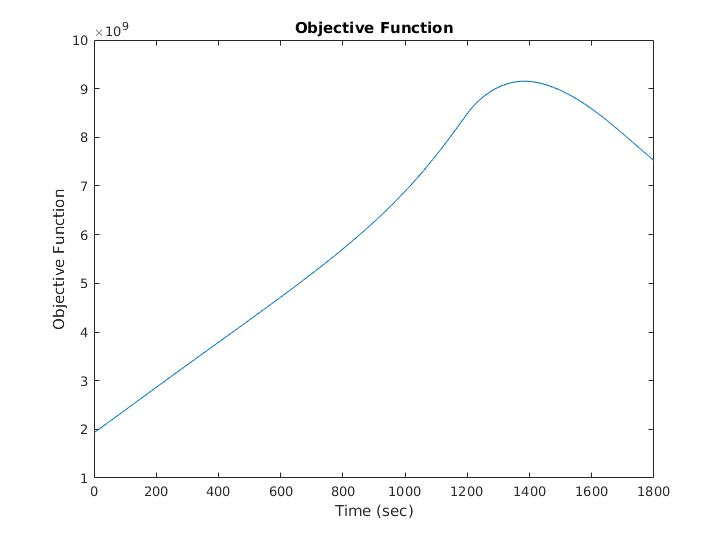
\includegraphics[width=4in]{objective.jpg}
\end{center}
\end{figure}
\begin{figure}[h!] 
\caption{Depicts the cooling profile for the controlled variable T(t) obtained at the final iteration}
\begin{center}
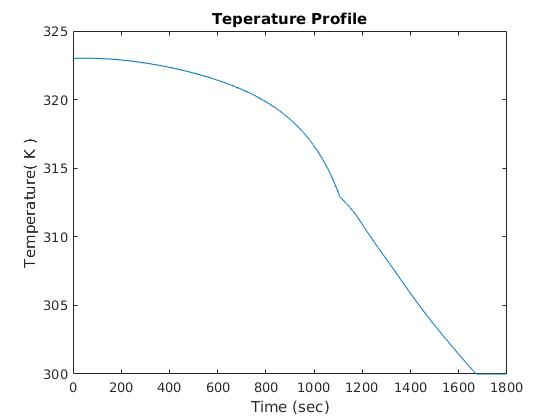
\includegraphics[width=4in]{temp.jpg}
\end{center}
\end{figure}
\clearpage
The change of the Hamiltonian Derivative($\frac{dH}{dT}$) after each iteration is shown below : 
\begin{figure}[h!]
  \centering
  \begin{minipage}[b]{0.4\textwidth}
    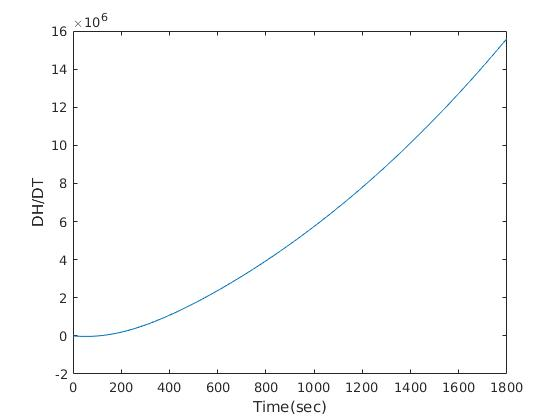
\includegraphics[width=\textwidth]{h1.jpg}
    \caption{Iteration 1}
  \end{minipage}
  \hfill
  \begin{minipage}[b]{0.4\textwidth}
    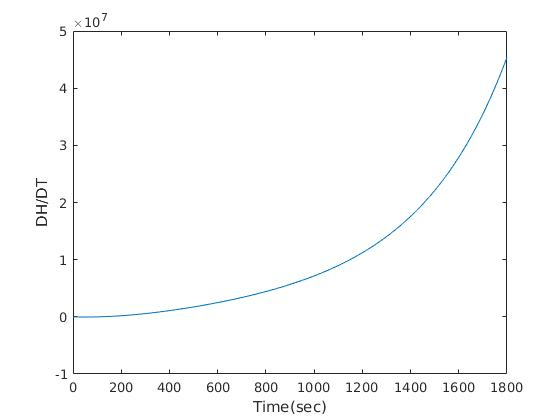
\includegraphics[width=\textwidth]{h2.jpg}
    \caption{Iteration 2}
  \end{minipage}
\end{figure}
\begin{figure}[h!]
  \centering
  \begin{minipage}[b]{0.4\textwidth}
    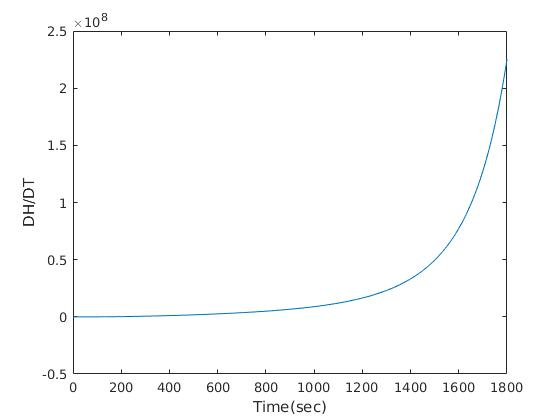
\includegraphics[width=\textwidth]{h3.jpg}
    \caption{Iteration 3}
  \end{minipage}
  \hfill
  \begin{minipage}[b]{0.4\textwidth}
    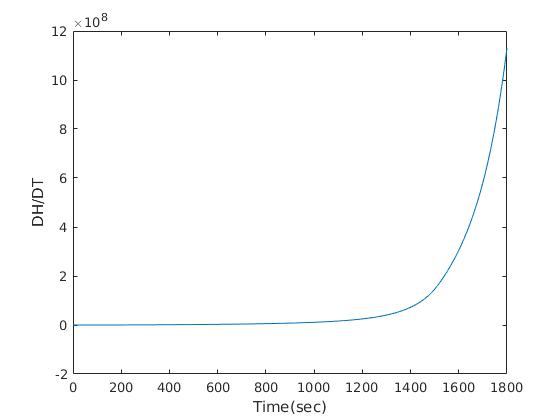
\includegraphics[width=\textwidth]{h4.jpg}
    \caption{Iteration 4}
  \end{minipage}
\end{figure}
\begin{figure}[h!]
  \centering
  \begin{minipage}[b]{0.4\textwidth}
    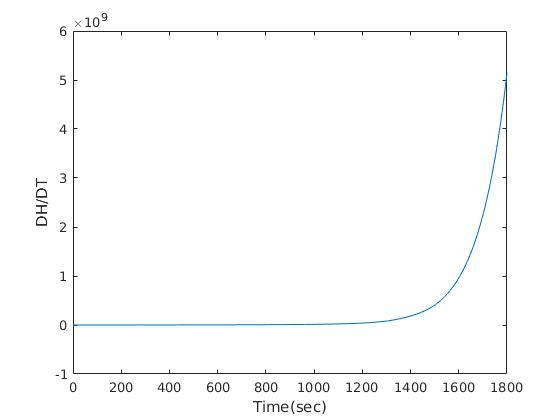
\includegraphics[width=\textwidth]{h5.jpg}
    \caption{Iteration 5}
  \end{minipage}
  \hfill
  \begin{minipage}[b]{0.4\textwidth}
    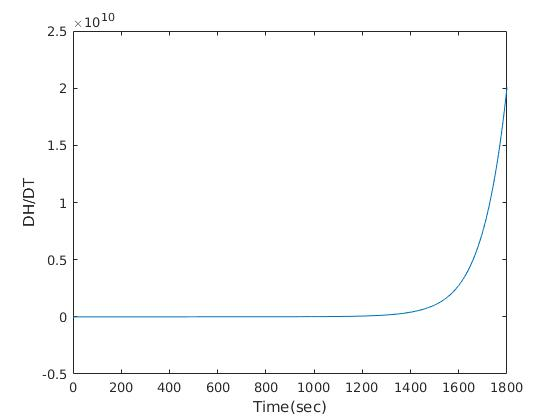
\includegraphics[width=\textwidth]{h6.jpg}
    \caption{Iteration 6}
  \end{minipage}
\end{figure} % Optimal Control Problems

%%% Uncertainity Quantification

\chapter{Optimal Control using Uncertainity Quantification}

\paragraph{Kinetic parameters} are generally empirical constants determined by fitting experimental data to the model, and, hence, are a source of uncertainty within the system. Two methods are discussed here to quantify these uncertainities and thereby perform build a more robust dynamic optimization.

\section{Stochastic Optimal Control using Ito Processes}

From several previous works it has been shown that the dynamic uncertainties
such as the batch reactors\cite{benavides2} and batch distillation,\cite{diwekar}, can be represented using stochastic processes called as the Ito processes.  We characterize the time-dependent uncertainties in the state variables using Ito processes.\\
The advantage lies in the ability to integrate the equations using the principles of stochastic calculus and the use of stochastic maximum principle to solve for the optimal temperature profile. \\
In batch crystallization kinetics, the growth and nucleation expressions have empirical constants shown in Table \ref{Table1}, they can be assumed to follow a Gaussian distribution\cite{yenkie}. By studying the nature of the dynamic uncertainty plots of the process variables and their correlation to Ito processes, it has been observed that the uncertainties can be best modeled with a simple Ito process known as \textbf{Brownian motion} with drift\cite{diwekar,wong}. It can be defined as:
\begin{equation} \label{gen}
dy = a(y,t)dt + b(y,t)dz
\end{equation}
where $dz$ is the increment of the Wiener process equal to $\varepsilon_{t}(\Delta t)^{1/2}$, and a(y,t) and b(y,t) are known functions. The random value $\varepsilon_{t}$  has a unit normal distribution with zero mean
and a standard deviation of 1. To estimate the values of the functions a and b, a generalized method presented by Diwekar\cite{diwekar} has been used.\\
In this work, equation(\ref{gen}) has been used to incorporate the uncertainties into the moment equations which are\cite{yenkie} :
\begin{align}
dy_{1} &= \left[-3\rho k_{v}G(t)(y_{4}+y{8})\right]\Delta t + g_{1}\varepsilon_{1}\sqrt{\Delta t} \\
dy_{2} &= 0 \\
dy_{3} &= (G(t)y_{2})\Delta t +g_{3}\varepsilon_{3}\sqrt{\Delta t} \\
dy_{4} &= (2G(t)y_{3})\Delta t + g_{4}\varepsilon_{4}\sqrt{\Delta t} \\
dy_{5} &= (3G(t)y_{4})\Delta t + g_{5}\varepsilon_{5}\sqrt{\Delta t} \\
dy_{6} &= (B(t))\Delta t + g_{6}\varepsilon_{6}\sqrt{\Delta t} \\
dy_{7} &= (G(t)y_{6})\Delta t + g_{7}\varepsilon_{7}\sqrt{\Delta t} \\
dy_{8} &= (2G(t)y_{7})\Delta t +g_{8}\varepsilon_{8}\sqrt{\Delta t} \\
dy_{9} &= (3G(t)y_{8})\Delta t + g_{9}\varepsilon_{9}\sqrt{\Delta t} \\
\end{align}
$a(y,t)$ in each equation is replaced by the corresponding deterministic function   for the state variable.\\
Here, the $g_{i}$ values represent the variance in the variable for which they are associated. They are calculated by recording the variance of the differences in $y_{i}$, which is divided by the time
interval $\Delta t$, and then the square root of this value is taken.


\paragraph{Objective Function} for the stochastic formulation now becomes :
\begin{equation} \label{objective}
\max_{T} L = \mathbf{E}\left[ \mu_{3}^{s}(t_{f}) - \mu_{3}^{n}(t_{f})\right]
\end{equation}
$\mathbf{E}$ is the expected value of the variable. \\
The \textbf{Active Constraints} and \textbf{Initial Conditions} remain the same as mentioned in Section (\ref{deterministic}).

\subsection{Solution Technique : Stochastic Steepest Ascent Hamiltonian}

The Hamiltonian for this section is modified to incorporate the uncertainities as\cite{yenkie} :
\begin{equation}
H = \sum_{i=1}^{9} \left( z_{i}f_{i} + \omega_{i}\frac{g_{y_{i}}^2}{2} \right)
\end{equation}
$f_{i}$ are the deterministic parts for the eq (5.2-5.11). $\omega_{i}$ is an additional adjoint variable defined to calculate the Hamiltonian for the \textbf{Stochastic Maximum Principle} formulation\cite{ramirez}.  

The \textbf{Algorithm} for the method remains same as mentioned in Section (4.1.1) with minor changes.
\begin{enumerate}
\item  Steps (1-4) are repeated. 
\item The variable θi corresponds to each of the state variable yi and the variable ∮ i corresponds to each of the adjoint variable zi , Ψi corresponding to each ωi respectively.
\item The variable $\theta_{i}$ corresponds to each of the state variable $y_{i}$ and the variable $\phi_{i}$ corresponds to each of the adjoint variable $z_{i}$, $\psi_{i}$ for each $\omega_{i}$ respectively.

\item The Hamiltonian derivative is now calculated at each time step  as :
\begin{align}
&\theta = \frac{dy_{i}}{dT} \quad \phi_{i} = \frac{dz_{i}}{dT} \quad \psi = \frac{d\omega_{i}}{dT} \\
&\frac{dH}{dT} = \sum_{i=1}^{9} \left( \frac{dH}{dy_{i}}\right)\left(	\frac{dy_{i}}{dT} \right) + \sum_{i=1}^{9} \left(\frac{dH}{dz_{i}}\right)\left(\frac{dz_{i}}{dT} \right) + \sum_{i=1}^{9} \left(\frac{dH}{dw_{i}}\right)\left(\frac{dw_{i}}{dT} \right)
\end{align}
\item The convergence criteria and the constraints remain same as the above referenced method.
\end{enumerate} 


\subsection{Results}
The following values were used as the coefficients for uncertainities for the state variables :
\begin{center}
\begin{table}[!h]
\centering
\caption{State Variable Uncertainity Coefficients\cite{yenkie}}
\begin{tabular}{|c|c|}
\hline
Parameters & Values \\
\hline
$g_{1}$ & $2.659\times10^{-5}$ \\
$g_{2}$ & $0$ \\
$g_{3}$ & $25.882$ \\
$g_{4}$ & $1.517\times10^{4}$ \\ 
$g_{5}$ & $6.57\times10^{6}$ \\
$g_{6}$ & $0.5486$ \\
$g_{7}$ & $25.9$\\
$g_{8}$ & $1382.34$ \\
$g_{9}$ & $8.753\times10^{4}$ \\
\hline
\end{tabular}

\label{Table2}
\end{table}
\end{center}

\begin{itemize}
\item The stochastic differential equations are integrated using stochastic calculus through \textbf{SDE Tools} Library available in \textbf{Matlab}.A strong Taylor approximation from the \textbf{Euler Maruyama} scheme has been used to integrate the equations which has an order of convergence of 0.5. 
\end{itemize}
The following profiles were obtained as a result :
\begin{figure}[h!] 

\begin{center}
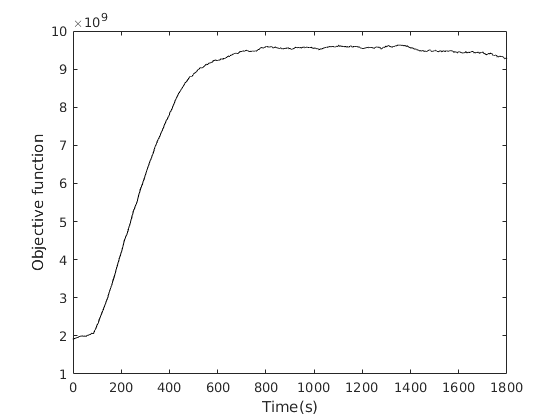
\includegraphics[width=4in]{Sobj.png}
\end{center}
\caption{Objective Function ($\mathbf{E}\left[\mu_{3}^{s}(t) - \mu_{3}^{n}(t)\right]$)}
\end{figure}
\begin{figure}[h!] 

\begin{center}
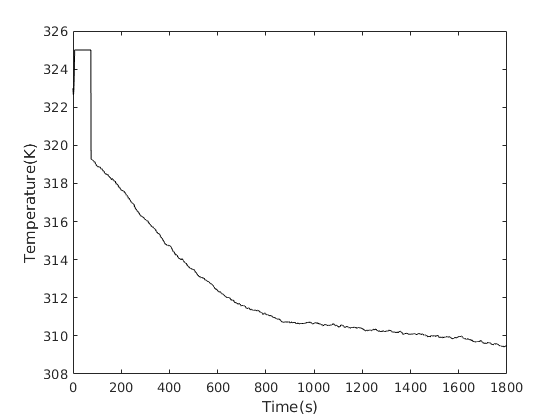
\includegraphics[width=4in]{Stemp.png}
\end{center}
\caption{The cooling profile for the controlled variable T(t) obtained at the final iteration}
\end{figure}

\begin{figure}[h!] 

\begin{center}
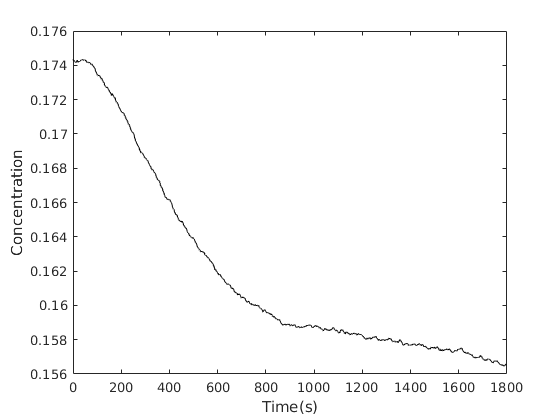
\includegraphics[width=4in]{Sconc.png}
\end{center}
\caption{Concentration Profile as obtained}
\end{figure}
\clearpage

\section{Stochastic Optimal Control using Polynomial Chaos Expansions}

\subsection{Introduction}
A Polynomial Chaos Expansion (PCE) describes a random process as a spectral expansion of random variables($\theta_{i}$), using orthogonal basis functions, $\Phi_{i}$ (Ghanem and Spanos, 1990,Ghanem and Spanos, 1997). For example, any second-order (finite variance) random process $y^{d}$, can be described using a PCE as follows:
\begin{equation}
y^{d} = a_{0}^{d}\phi_{0} + \sum_{i_{1}=1}^{\infty} a_{i_{1}}^{d}\phi_{1}(\theta_{i_{i1}}) + \sum_{i_{1}=1}^{\infty}\sum_{i_{2}=1}^{i_{1}} a_{i_{1}i_{2}}^d\phi_{2}(\theta_{i_{1}},\theta_{i_{2}})
\end{equation}
where $a_{i_{1}}^d$  are deterministic coefficients for each term in the expansion. The number of independent sources of random variables $(\theta_{i_{1}}, \theta_{i_{2}})$, generally defines the dimensionality, $n_{0}$. For practical application these expansions can be
truncated to a finite number of terms. Then the maximum polynomial order for the basis function, q needs to be defined.
The number of terms now become $P_{PCE} = \frac{(n_{0}+q)!}{n_{0}!q!} -1 $. \\
Using these notations a truncated PCE expansion can be represented as follows:
\begin{equation} 
\label{poly}
y^{d} \approx \sum_{i=1}^{P_{PCE}} a_{i}^{d}\phi_{\theta}
\end{equation}

The orthogonality property of the basis functions($\phi_{i}$) is used for the  calculation of the coefficients when propagating uncertainty from the input random variables$(\theta_{i_{1}}, \theta_{i_{2}})$, to the output random
variables ($y^{d}$).\\
The choice of the basis functions $\phi_{i}$ depends on the type of stochastic distribution to be represented, i.e. normal or uniform. In our case the parameters follow a Gaussian distribution\cite{yenkie}, which uses Hermite Polynomials to describe the probability distribution in the least number of terms.\\
Thus, given a process model with uncertain output, $y = X(x,\lambda)$, where $x$ is the uncertain input and $\lambda$ is the uncertain parameter, the aim is to quantify uncertainty in $y(\theta)$ from $x(\theta), \lambda(\theta)$ using the process model. Then the first step is to construct PCE’s of $x(\theta)$, and $\lambda(\theta)$, by determining their PCE coefficients $x_{i}$ and $\lambda_{i}$.
\begin{align}
&x(\theta) = \sum_{i=1}^{P_{PCE}} x_{i}\phi(\theta)
&\lambda(\theta) = \sum_{i=1}^{P_{PCE}} \lambda_{i}\phi(\theta)
\end{align}
\begin{equation}
&x_{i} = \frac{\int x\phi_{i}(\theta)g(\theta) d\theta}{\left\langle \phi^{2}_{i}\right\rangle } \quad
&\lambda_{i} = \frac{\int \lambda\phi_{i}(\theta)g(\theta) d\theta}{\left\langle \phi^{2}_{i}\right\rangle }
\end{equachaospytion}
where $g(\theta)$ is probability distribution function (pdf) of $\theta$. 
The next step is to develop PCE for $y(\theta)$ from  $x(\theta)$, and $\lambda(\theta)$, which can be done by evaluating the
inner product of $y(\theta)$ with each basis functions $\phi_{i}$ to determine the ith- PCE coefficient.
\begin{equation}
y_{i} = \frac{\left\langle f(x,\lambda)\phi_{i} \right\rangle }{\left\langle \phi^{2}_{i} \right\rangle }
\end{equation}
Evaluating the inner product $\left\langle y\phi_{i} \right\rangle $, requires computation of multi-dimensional integrals which can be performed by one of two approaches referred to as \textbf{non-intrusive} and \textbf{intrusive}.\\
The work under consideration here uses a non-intrusive approach. The model $y=X(x,\lambda)$ is represented by the modelling equations of Section(\ref{modeleq}). $x$ are the state variables and $\lambda$'s are the kinetic parameters.

\subsection{Usage of PCE in Batch Crystallization}

The model under consideration is composed of the state equations and kinetics mentioned in Section(\ref{modeleq}), which are :

\begin{align} 
\frac{dy_{1}}{dt} &= -3\rho k_{v}G(t)(y_{4}+y{8}) \\
\frac{dy_{2}}{dt} &= 0 \\
\frac{dy_{3}}{dt} &= G(t)y_{2}  \\
\frac{dy_{4}}{dt} &= 2G(t)y_{3} \\
\frac{dy_{5}}{dt} &= 3G(t)y_{4} \\
\frac{dy_{6}}{dt} &= B(t)  \\
\frac{dy_{7}}{dt} &= G(t)y_{6}  \\
\frac{dy_{8}}{dt} &= 2G(t)y_{7}  \\
\frac{dy_{9}}{dt} &= 3G(t)y_{8}  \\
\end{align}  

Here, the state varibles($y_{i}$) act as the uncertain outputs which is caused by errors in process parameters used to calculate the Growth rate ($G(t) = k_{g}\exp{\left(-E_{g}/RT \right)}\left(\frac{C - C_{s}(T)}{C_{s}(T)}\right)^{g}$) and the Nucleation rate ($B(t) = k_{b}\exp{\left(-E_{b}/RT \right)}\left(\frac{C - C_{s}(T)}{C_{s}(T)}\right)^{b}\mu_{3}$). As a result, uncertainities in the parameters $\lambda$ ($k_{g}, E_{g}, g, k_{b}, E_{b}, b$) are propogated into the model using P.C.E during optimal control.\\
A non-intrusive approach is followed for the above task where the integrals are calculated by generating samples of the above process and evaluating the model at these pre-determined points.
\paragraph{Algorithm} is as follows : 
\begin{enumerate}
\item Following the general representation, $y_{i}$ can be written as :
\begin{align*}
y_{i} = f(x(\theta),\lambda_{i}(\theta))
\end{align*}
where x is the input temperature(T), $\lambda_{i}$'s are process the parameters and $\theta$ is the random variable.
%% Can add a example expression here
\item The process model consists of 6 uncertainities which computationally prohibits the evaluation. Thus, an approximation of $n_{0} = 2$ is taken by employing a joint distribution of the parameters.
\item Samples are generated for the model at $N$ points. The sampling technique used is the Gaussian Quadratures along with Hermite Polynomials to represent state variables $(y_{i})$ into Eq(5.17).

\item For each of the above sample $y^{j}_{i} = f(T^{j}(\theta),\lambda(\theta) $ ,  the optimization problem is solved using the Steepest Ascent Hamiltonian method discussed in Section(4.1.1).

\item The optimum value of the input temperature $T^{j}(\theta)$ at these samples is used to construct the PCE's for $T(\theta)$ and $\lambda(\theta)$ as given by Equations(5.18).

\item $y^{j}_{i}$'s for each sample are used to evaluate :
\begin{equation}
y_{i} = \frac{1}{\left\langle \phi^{2}_{i}\right\rangle }\frac{1}{N} \sum_{j=1}^{N} y^{j}\phi_{i}(\theta)
\end{equation}
Here, $\phi_{i}$ are the coefficients of the orthogonal polynomials being used for PCE estimation.  

\item As the above Equation averages over N samples, the resultant $y_{i}$ maximises the objective function, given by $ \mathbf{E} \left\lbrace  y_{5}-y_{9} \right\rbrace $). 

\end{enumerate} 

The kinetic parameter values used for the above model are given below :
\begin{center}
\begin{table}[!h]
\centering
\caption{Kinetic Parameter Uncertainities\cite{hu,shi,paeng}}
\begin{tabular}{|c|c|c|}
\hline
Parameters & Experimental Values & Range of Values\\
\hline
\multicolumn{3}{|c|}{Growth Kinetics} \\
\hline
$k_{g}$ & $1.44\times10^{8} \mu m s^{-1}$ & $1.368 - 1.512\times10^{8} $\\
$E_{g}/R$ & $4859K$ & $4606.15-5101.95$\\
$g$ & $1.5$ & $1.425-1.575$\\
\hline
\multicolumn{3}{|c|}{Nucleation Kinetics} \\
\hline
$k_{b}$ & $285 (s \mu m^{3})^{-1}$ & $270.75-299.25$\\ 
$E_{b}/R$ & $7517K$ & $7141.15-7892.85$\\
$b$ & $1.45$ & $1.3775-1.5225$\\
\hline
\end{tabular}

\label{Table3}
\end{table}
\end{center}



\subsection{Results}

\begin{itemize}
\item The method was implemented in pyhton using the \textbf{chaospy} library\cite{chaospy} for Polynomial Chaos Expnasions. 
\end{itemize}
The following profiles were obtained : 

\begin{figure}[h!] 

\begin{center}
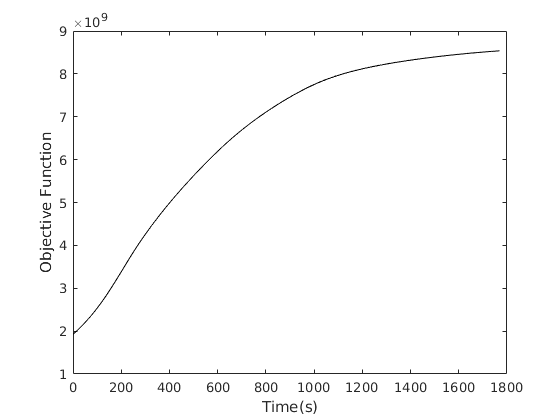
\includegraphics[width=4in]{PCEobj.png}
\end{center}
\caption{Objective Function ($\mathbf{E}\left[\mu_{3}^{s}(t) - \mu_{3}^{n}(t)\right]$)}
\end{figure}
\begin{figure}[h!] 

\begin{center}
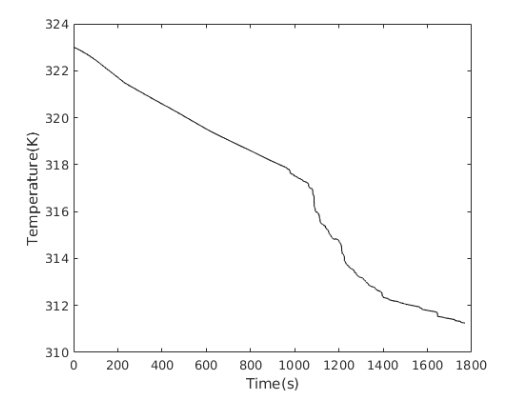
\includegraphics[width=4in]{PCETemp2.png}
\end{center}
\caption{The cooling profile for the controlled variable T(t) obtained at the final iteration}
\end{figure}

\begin{figure}[h!] 

\begin{center}
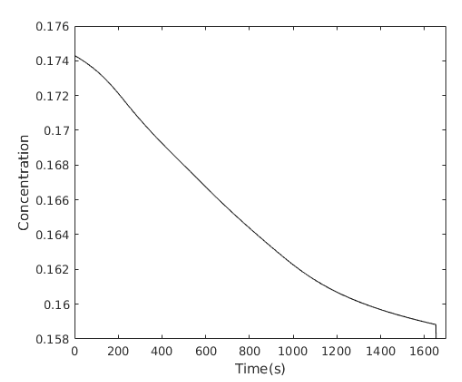
\includegraphics[width=4in]{PCEConc.png}
\end{center}
\caption{The concentration profile as obtained.}
\end{figure}
\clearpage

\section{Conclusions}
\begin{itemize}
\item The same process was optimized using 3 different methods of Optimization. This achieves the aim of maximising the volume of the product obtained. 
\item The Temperature profile for all the 3 cases was obtained as a decreasing one and thus follows the principle of batch cooling crystallization. 
\item Polynomial Chaos Expansions, when applied to crystallization performs at par with the existing methods in optimizing the process by efficiently incorporating uncertainities. 
\item After comparing the final values of the objective functions($\mu_{3}^{s}-\mu_{3}^{n}$)[particle volume] the following values were obtained : 
\begin{enumerate}
\item Deterministic : $ 9.153 \times 10^{9} \mu m^{3}$
\item Expected value for Stochastic involving Ito Processes : $8.978 \times 10^{9} \mu m^{3}$
\item Expected value for Stochastic case involving PCE : $8.64 \times 10^{9} \mu m^{3}$
\end{enumerate}
\item The decrease of values can be attributed to the presence of errors or uncertainities in the kinetic parameters. Thus, the model becomes helpful in predicting the expected values for volume of crystals taking care of the process uncertainities.
\end{itemize} % Stochastic and PCE 

\chapter{Stochastic Optimization using Polynomial Chaos Expansions : Unseeded Crystallization}

\paragraph{Aim} To build a predictive model for unseeded batch crystallization of L-Asparagine Monohyrdate(LAM). 


\section{Optimal Control Problem}

The population balance equations(PBE) given by \ref{populationbalance} are used here to model the kinetics of crystal formation. The Nucleation rate expression for LAM crystals is given by\cite{lindenberg} :
\begin{equation}
B = k_{j_{1}}S\exp\left( -k_{j_{2}}\frac{\ln^{3}{C_{c}/C^{*}}}{\ln^{2}S}\right) 
\end{equation}
$C_{c}$ representys the  molar density of LAM. kJ1 and kJ2 are
empirical parameters. The following power-law expression is used to describe the growth rate\cite{nagy}\cite{nagy2}:
\begin{equation}
G = k_{g}(S-1)^{g}
\end{equation}
The supersaturation ratio, S, is defined as :
\begin{equation}
S = C/C^{*}
\end{equation}
C* represents the saturation concentration of LAM. The solubility of LAM in 
can be expressed as:
\begin{equation}
C^{*} = 5 \times 10^{-5}T^{2} - 0.001T + 0.0236
\end{equation}
Method of Moments has been used to reduce the PBE to ODE's as stated in Section \ref{modeleq}. The mass balance for LAM crystals also remains the same from there, with the difference being the absence of seeded crystals.\\
The ODEs for the model are given by :
\begin{align}
\frac{du_{0}}{dt} &= B \\
\frac{du_{j}}{dt} &= jG\mu_{j-1}
\end{align}
for  $j = 1,2,3,4 $
\\
The determination of the optimal temperature profile for maximizing the weight mean size is a highly studied objective for a crystallization process.Thus, 
\paragraph{Objective Function} becomes :
\begin{align}
\max_{T(t)}	\phi = \mu_{4}/\mu_{3} \quad at \quad t_{f} 
\end{align}
\paragraph{Constraints}
\begin{align}
T_{min} &\leqslant T(t) \leqslant T_{max} \\
\frac{dT}{dt} &\leqslant 0
\end{align}
The state variables can be represented as :
\begin{equation*}
y_{i} = \left[\quad C \quad \mu_{0} \quad \mu_{1} \quad \mu_{2} \quad \mu_{3}\quad \mu_{4} \quad\right]  
\end{equation*}
Here we do not divide the moments in seeded and nucleated ones.\\
The Hamiltonian method described in the previous sections was employed to solve the optimaization problem along with the uncertainity quantification being done using Polynomial Chaos Expansions. The new state equations, constraints and kinetics as described above are used to define the problem.\\

\section{Solution Technique : Hamiltonian Steepest Ascent with PCE}

Equations(6.5-6.6) take place as the new state equations and the uncertain parameters are mentioned in Table 6.1. The constraint(Eq 6.9)) depicts a cooling profile for the crystallizer. The obejective function here (Eq 6.7) differs from the one used in Section(\ref{deterministic}) so as to calculate the final maximum mean size of the crystals.\\ 
Key Differences :
\begin{itemize}
\item The batch time for the model was taken to be 240 min($t_{f}$).
\item An initial concentration value of 0.073 $g/L$ was taken to obtain the cooling profile. All the moments were intialised to 0.
\item The ODEs were integrated using Python \textbf{scipy's} \textbf{odeint} integrator.
\end{itemize}

\begin{center}
\begin{table}[!h]
\centering 
\caption{Kinetic Parameters\cite{bhoi}}
\begin{tabular}{|c|c|c|}
\hline
Parameters & Experimental Values & Range of Values\\
\hline
\multicolumn{3}{|c|}{Growth Kinetics} \\
\hline
$\ln(k_{g})$ & $3.41\pm 0.28 & \mu m min^{-1} $\\
$g$ & $1.48\pm 0.04$ & $ - $\\
\hline
\multicolumn{3}{|c|}{Nucleation Kinetics} \\
\hline
$\ln(k_{j_{1}})$ & $24.74\pm0.73$ & $No. per m^{3}min$\\ 
$k_{j_{2}}$ & $2.7\times10^{-2}\pm 3.2\times10^{-3}$ & $-$\\
\hline
\end{tabular}

\label{values}
\end{table}
\end{center}

\paragraph{Algorithm}
\begin{enumerate}
\item The process model consists of 4 uncertainities which computationally prohibits the evaluation. Thus, the experiment has been done on $k_{g}$ and $g$, employing a joint distribution of the parameters.
\item Samples are generated using the distribution using Gaussian Quadrature Scheme.
\item The function is evaluated at each of these samples to evalute the integrals numerically to determine the PCE coefficients.
\item At each sample, optimization of the model is performed using the Determinstic Approach explained in Section(\ref{deterministic}).
\item The convergence criteria and the constraints remain same as the above referenced method.
\end{enumerate}

\section{Results}
The value for the concentration profile for the time horizon was obtained as :
\begin{figure}[h!] 
\begin{center}
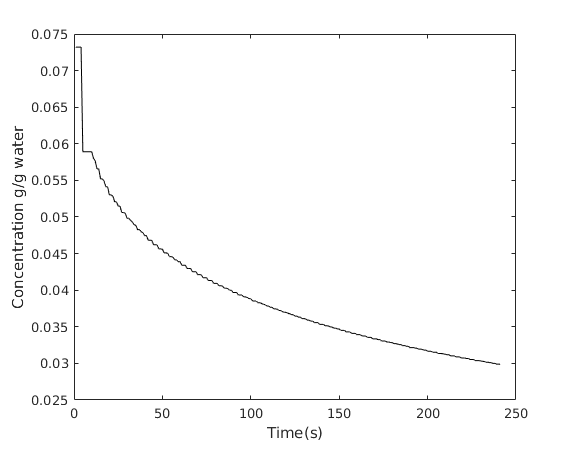
\includegraphics[width=4in]{AppConc.png}
\end{center}
\caption{Concentration Profile}
\end{figure}

The value for the temperature profile was obtained as :
\begin{figure}[h!] 
\begin{center}
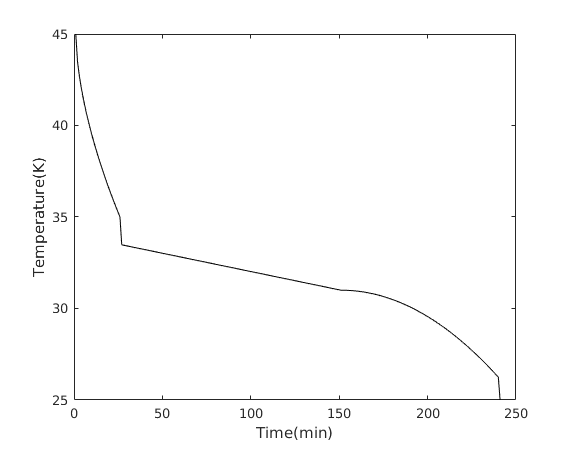
\includegraphics[width=4in]{AppTemp.png}
\end{center}
\caption{Temperature Profile}
\end{figure}

\section{Conclusion}

\begin{itemize}
\item The final value of the objective function($\mu_{4}/\mu_{3}$), ie. the mean crystal size was obtained at : $300 \mu m$
\item The model performs at par with other cooling policies such as cubic cooling policy($251 \mu m$)\cite{bhoi}. This proves the efficacy of P.C.E in the field of batch crystallization.
\end{itemize}
 % Results and Discussion

%\input{Chapters/Chapter7} % Conclusion

%% ----------------------------------------------------------------
% Now begin the Appendices, including them as separate files

\addtocontents{toc}{\vspace{2em}} % Add a gap in the Contents, for aesthetics

%\appendix % Cue to tell LaTeX that the following 'chapters' are Appendices

%\chapter{An Appendix}

Lorem ipsum dolor sit amet, consectetur adipiscing elit. Vivamus at pulvinar nisi. Phasellus hendrerit, diam placerat interdum iaculis, mauris justo cursus risus, in viverra purus eros at ligula. Ut metus justo, consequat a tristique posuere, laoreet nec nibh. Etiam et scelerisque mauris. Phasellus vel massa magna. Ut non neque id tortor pharetra bibendum vitae sit amet nisi. Duis nec quam quam, sed euismod justo. Pellentesque eu tellus vitae ante tempus malesuada. Nunc accumsan, quam in congue consequat, lectus lectus dapibus erat, id aliquet urna neque at massa. Nulla facilisi. Morbi ullamcorper eleifend posuere. Donec libero leo, faucibus nec bibendum at, mattis et urna. Proin consectetur, nunc ut imperdiet lobortis, magna neque tincidunt lectus, id iaculis nisi justo id nibh. Pellentesque vel sem in erat vulputate faucibus molestie ut lorem.

Quisque tristique urna in lorem laoreet at laoreet quam congue. Donec dolor turpis, blandit non imperdiet aliquet, blandit et felis. In lorem nisi, pretium sit amet vestibulum sed, tempus et sem. Proin non ante turpis. Nulla imperdiet fringilla convallis. Vivamus vel bibendum nisl. Pellentesque justo lectus, molestie vel luctus sed, lobortis in libero. Nulla facilisi. Aliquam erat volutpat. Suspendisse vitae nunc nunc. Sed aliquet est suscipit sapien rhoncus non adipiscing nibh consequat. Aliquam metus urna, faucibus eu vulputate non, luctus eu justo.

Donec urna leo, vulputate vitae porta eu, vehicula blandit libero. Phasellus eget massa et leo condimentum mollis. Nullam molestie, justo at pellentesque vulputate, sapien velit ornare diam, nec gravida lacus augue non diam. Integer mattis lacus id libero ultrices sit amet mollis neque molestie. Integer ut leo eget mi volutpat congue. Vivamus sodales, turpis id venenatis placerat, tellus purus adipiscing magna, eu aliquam nibh dolor id nibh. Pellentesque habitant morbi tristique senectus et netus et malesuada fames ac turpis egestas. Sed cursus convallis quam nec vehicula. Sed vulputate neque eget odio fringilla ac sodales urna feugiat.

Phasellus nisi quam, volutpat non ullamcorper eget, congue fringilla leo. Cras et erat et nibh placerat commodo id ornare est. Nulla facilisi. Aenean pulvinar scelerisque eros eget interdum. Nunc pulvinar magna ut felis varius in hendrerit dolor accumsan. Nunc pellentesque magna quis magna bibendum non laoreet erat tincidunt. Nulla facilisi.

Duis eget massa sem, gravida interdum ipsum. Nulla nunc nisl, hendrerit sit amet commodo vel, varius id tellus. Lorem ipsum dolor sit amet, consectetur adipiscing elit. Nunc ac dolor est. Suspendisse ultrices tincidunt metus eget accumsan. Nullam facilisis, justo vitae convallis sollicitudin, eros augue malesuada metus, nec sagittis diam nibh ut sapien. Duis blandit lectus vitae lorem aliquam nec euismod nisi volutpat. Vestibulum ornare dictum tortor, at faucibus justo tempor non. Nulla facilisi. Cras non massa nunc, eget euismod purus. Nunc metus ipsum, euismod a consectetur vel, hendrerit nec nunc.	% Appendix Title

%\input{Appendices/AppendixB} % Appendix Title

%\input{Appendices/AppendixC} % Appendix Title

\addtocontents{toc}{\vspace{2em}}  % Add a gap in the Contents, for aesthetics
\backmatter

%%

\begin{thebibliography}{9}
\bibitem{mullin}
Mulin, J. W.; Nyvlt, J. Programmed cooling of batch crystallizers.
\textit{Chem. Eng. Sci.} \textbf{1971}, \textit{26}, 369−377.

\bibitem{agjones}
Jones, A. G. Optimal operation of a batch cooling crystallizer.
\textit{Chem. Eng. Sci.} \textbf{1974}, \textit{29}, 1075−1087.
\bibitem{rawlings}
 Rawlings, J. B.; Witkowski, W. R.; Eaton, J. W. Modeling and
control of crystallizers.\textit{ Powder Technol.} \textbf{1992}, \textit{69}, 3−9.
\bibitem{miller_rawlings}
 Miller, S. M.; Rawlings, J. B. Model identification and control
strategies for batch cooling crystallizers. \textit{AIChE J.} \textbf{1994}, \textit{40}, 1312−
1327.
\bibitem{hu}
Hu, Q.; Rohani, S.; Jutan, A. Modelling and optimization of
seeded batch crystallizers. \textit{Comput. Chem. Eng.} \textbf{2005}, \textit{29}, 911−918.

\bibitem{shi}
Shi, D.; El-Farra, N.; Li, M.; Mhaskar, P.; Christofides, P. D.
Predictive control of particle size distribution in particulate processes.
\textit{Chem. Eng. Sci.} \textbf{2006}, \textit{61}, 268−28.

\bibitem{paeng}
Paengjuntuek, W.; Arpornwichanop, A.; Kittisupakorn, P.
Product quality improvement of batch crystallizers by a batch to
batch optimization and non-linear control approach. \textit{Chem. Eng. J.}
\textbf{2008}, \textit{139}, 344−350.

\bibitem{diwekar}
Diwekar, U. \textit{Introduction to Applied Optimization}, 2nd ed.;
Springer: New York, 2008
\bibitem{benavides}
Benavides, P. T.; Diwekar, U. Optimal control of biodiesel
production in a batch reactor. Part I: Deterministic control. Fuel \textbf{2011}, DOI: 10.1016/j.fuel.2011.08.035.
\bibitem{yenkie}
Yenkie, K. M., & Diwekar, U. Stochastic optimal control of seeded batch crystallizer applying the ito process. \textit{Industrial & Engineering Chemistry Research}, \textbf{2012}, \textit{52(1)}, 108-122.
\bibitem{wong}
Wong, E.; Zakai, M. On the relation between ordinary and
stochastic differential equations. \textit{Int. J. Eng. Sci.} \textbf{1965}, \textit{3}, 213−229.
\bibitem{corriou}
Corriou, J. P.; Rohani, S. A new look at optimal control of a
batch crystallizer. \textit{AIChE J.},\textbf{2008}, \textit{54}, 3188−3206.
\bibitem{grosso}
Grosso, M.; Cogoni, G.; Baratti, R.; Romagnoli, J. A. Stochastic
Approach for the prediction of PSD in crystallization processes:
Formulation and comparative assessment of different stochastic
models. \textit{Ind. Eng. Chem. Res.}, \textbf{2011}, \textit{50}, 2133−2143.
\bibitem{ma}
Ma, D. L.; Chung, S. H.; Braatz, R. D. Worst-case performance
analysis of optimal batch control trajectories. \textit{AIChE J.} \textbf{1999}, \textit{45}, 1469−1476.
\bibitem{benavides2}
Benavides, P. T.; Diwekar, U. Optimal control of biodiesel
production in a batch reactor. Part II: Stochastic control. \textit{Fuel} \textbf{2012}, \textit{94}, 218−226.
\bibitem{ramirez}
Rico-Ramirez, V.; Diwekar, U. M. Stochastic maximum principle
for optimal control under uncertainty. \textit{Comput. Chem. Eng.} \textbf{2004}, \textit{28}, 2845−2849
\bibitem{chaospy}
Feinberg, J., & Langtangen, H. P. Chaospy: An open source tool for designing methods of uncertainty quantification. \textit{Journal of Computational Science},\textbf{2015}, \textit{11}, 46-57.
\bibitem{lindenberg}
C. Lindenberg and M. Mazzotti,\textit{ AIChE J.}, \textbf{2011}, \textit{57}, 942–950.
\bibitem{nagy}
 Z. Nagy,\textit{ Comput. Chem. Eng.}, \textbf{2009}, \textit{33}, 1685–1691.
\bibitem{nagy2}
 Z. Nagy, M. Fujiwara, X. Woo and R. Braatz,\textit{ Ind. Eng. Chem.
Res.},\textbf{ 2008}, \textit{47}, 1245–1252.
\bibitem{bhoi}
Bhoi, Stutee, Maheswata Lenka, and Debasis Sarkar. "Particle engineering by optimization for the unseeded batch cooling crystallization of L-asparagine monohydrate." \textit{CrystEngComm 19.42} \textbf{(2017)}, 6373-6382.

\end{thebibliography}
 ----------------------------------------------------------------
\label{Bibliography}
\lhead{\emph{Bibliography}}  % Change the left side page header to "Bibliography"
\bibliographystyle{unsrtnat}  % Use the "unsrtnat" BibTeX style for formatting the Bibliography
\bibliography{Bibliography}  % The references (bibliography) information are stored in the file named "Bibliography.bib"

\end{document}  % The End
%% ----------------------------------------------------------------